% Time form: Past tense

\newpage
\section{Workshops}\label{sec:workshops}

In the Project Management phase, several workshops were conducted, including a brainstorming session using Post-it notes and a User Story Mapping exercise on a whiteboard.
The goal of these workshops was to clarify the scenarios a network edge device should support.

Following these workshops, the insights gathered were used to derive issues and goals, which were then mapped to detailed milestones in GitLab.
All deliverables were categorized using the MoSCoW prioritization method into must, should, and could requirements.
An example of this prioritization and scenario mapping is illustrated in Figure~\ref{fig:usm-network-discovery}.
All Milestones links are provided in the URL at the top of the section.

\subsection{Brainstorm Scenario Selection}\label{subsec:brainstorm-scenario-selection}

In this workshop, participants brainstorm and cluster potential red and blue team scenarios for practical cybersecurity exercises.

\begin{figure}[H]
	\centering
	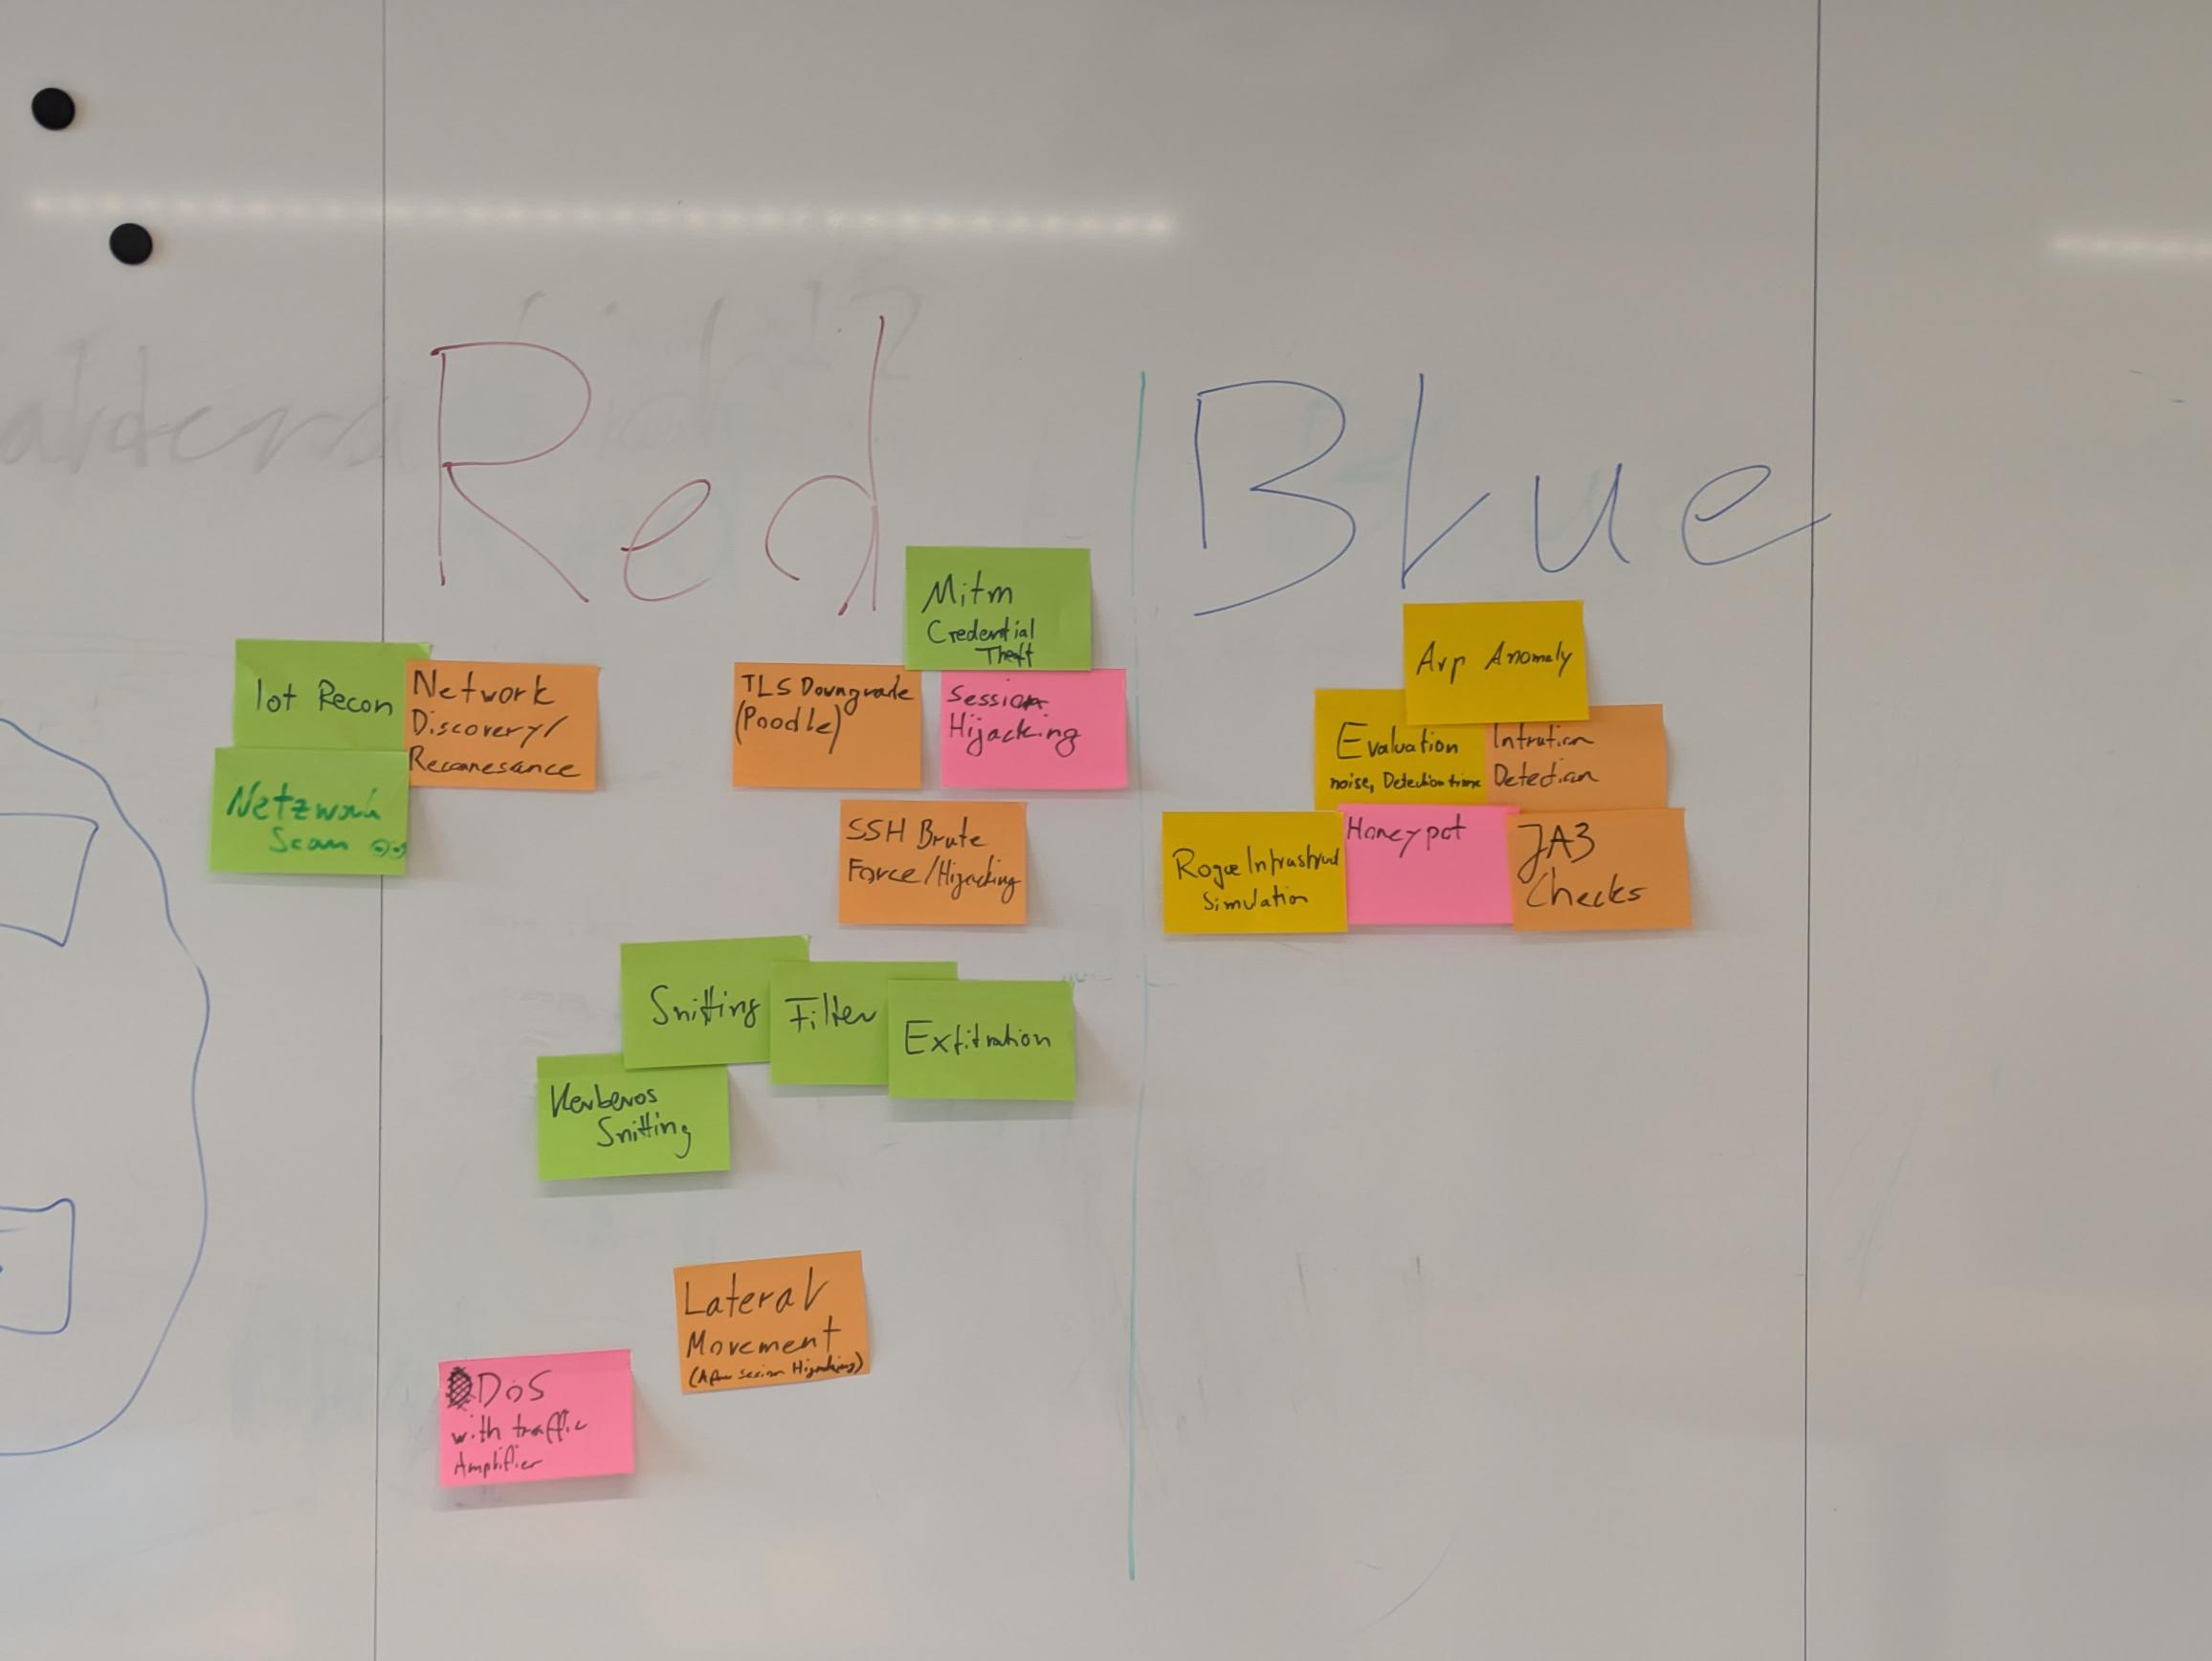
\includegraphics[width=1.0\linewidth]{appendix/appendix-media/Workshops/brainstorm-scenarios}
	\caption{Brainstorm Scenarios}
	\label{fig:brainstorm-scenarios}
\end{figure}

\begin{figure}[H]
	\centering
	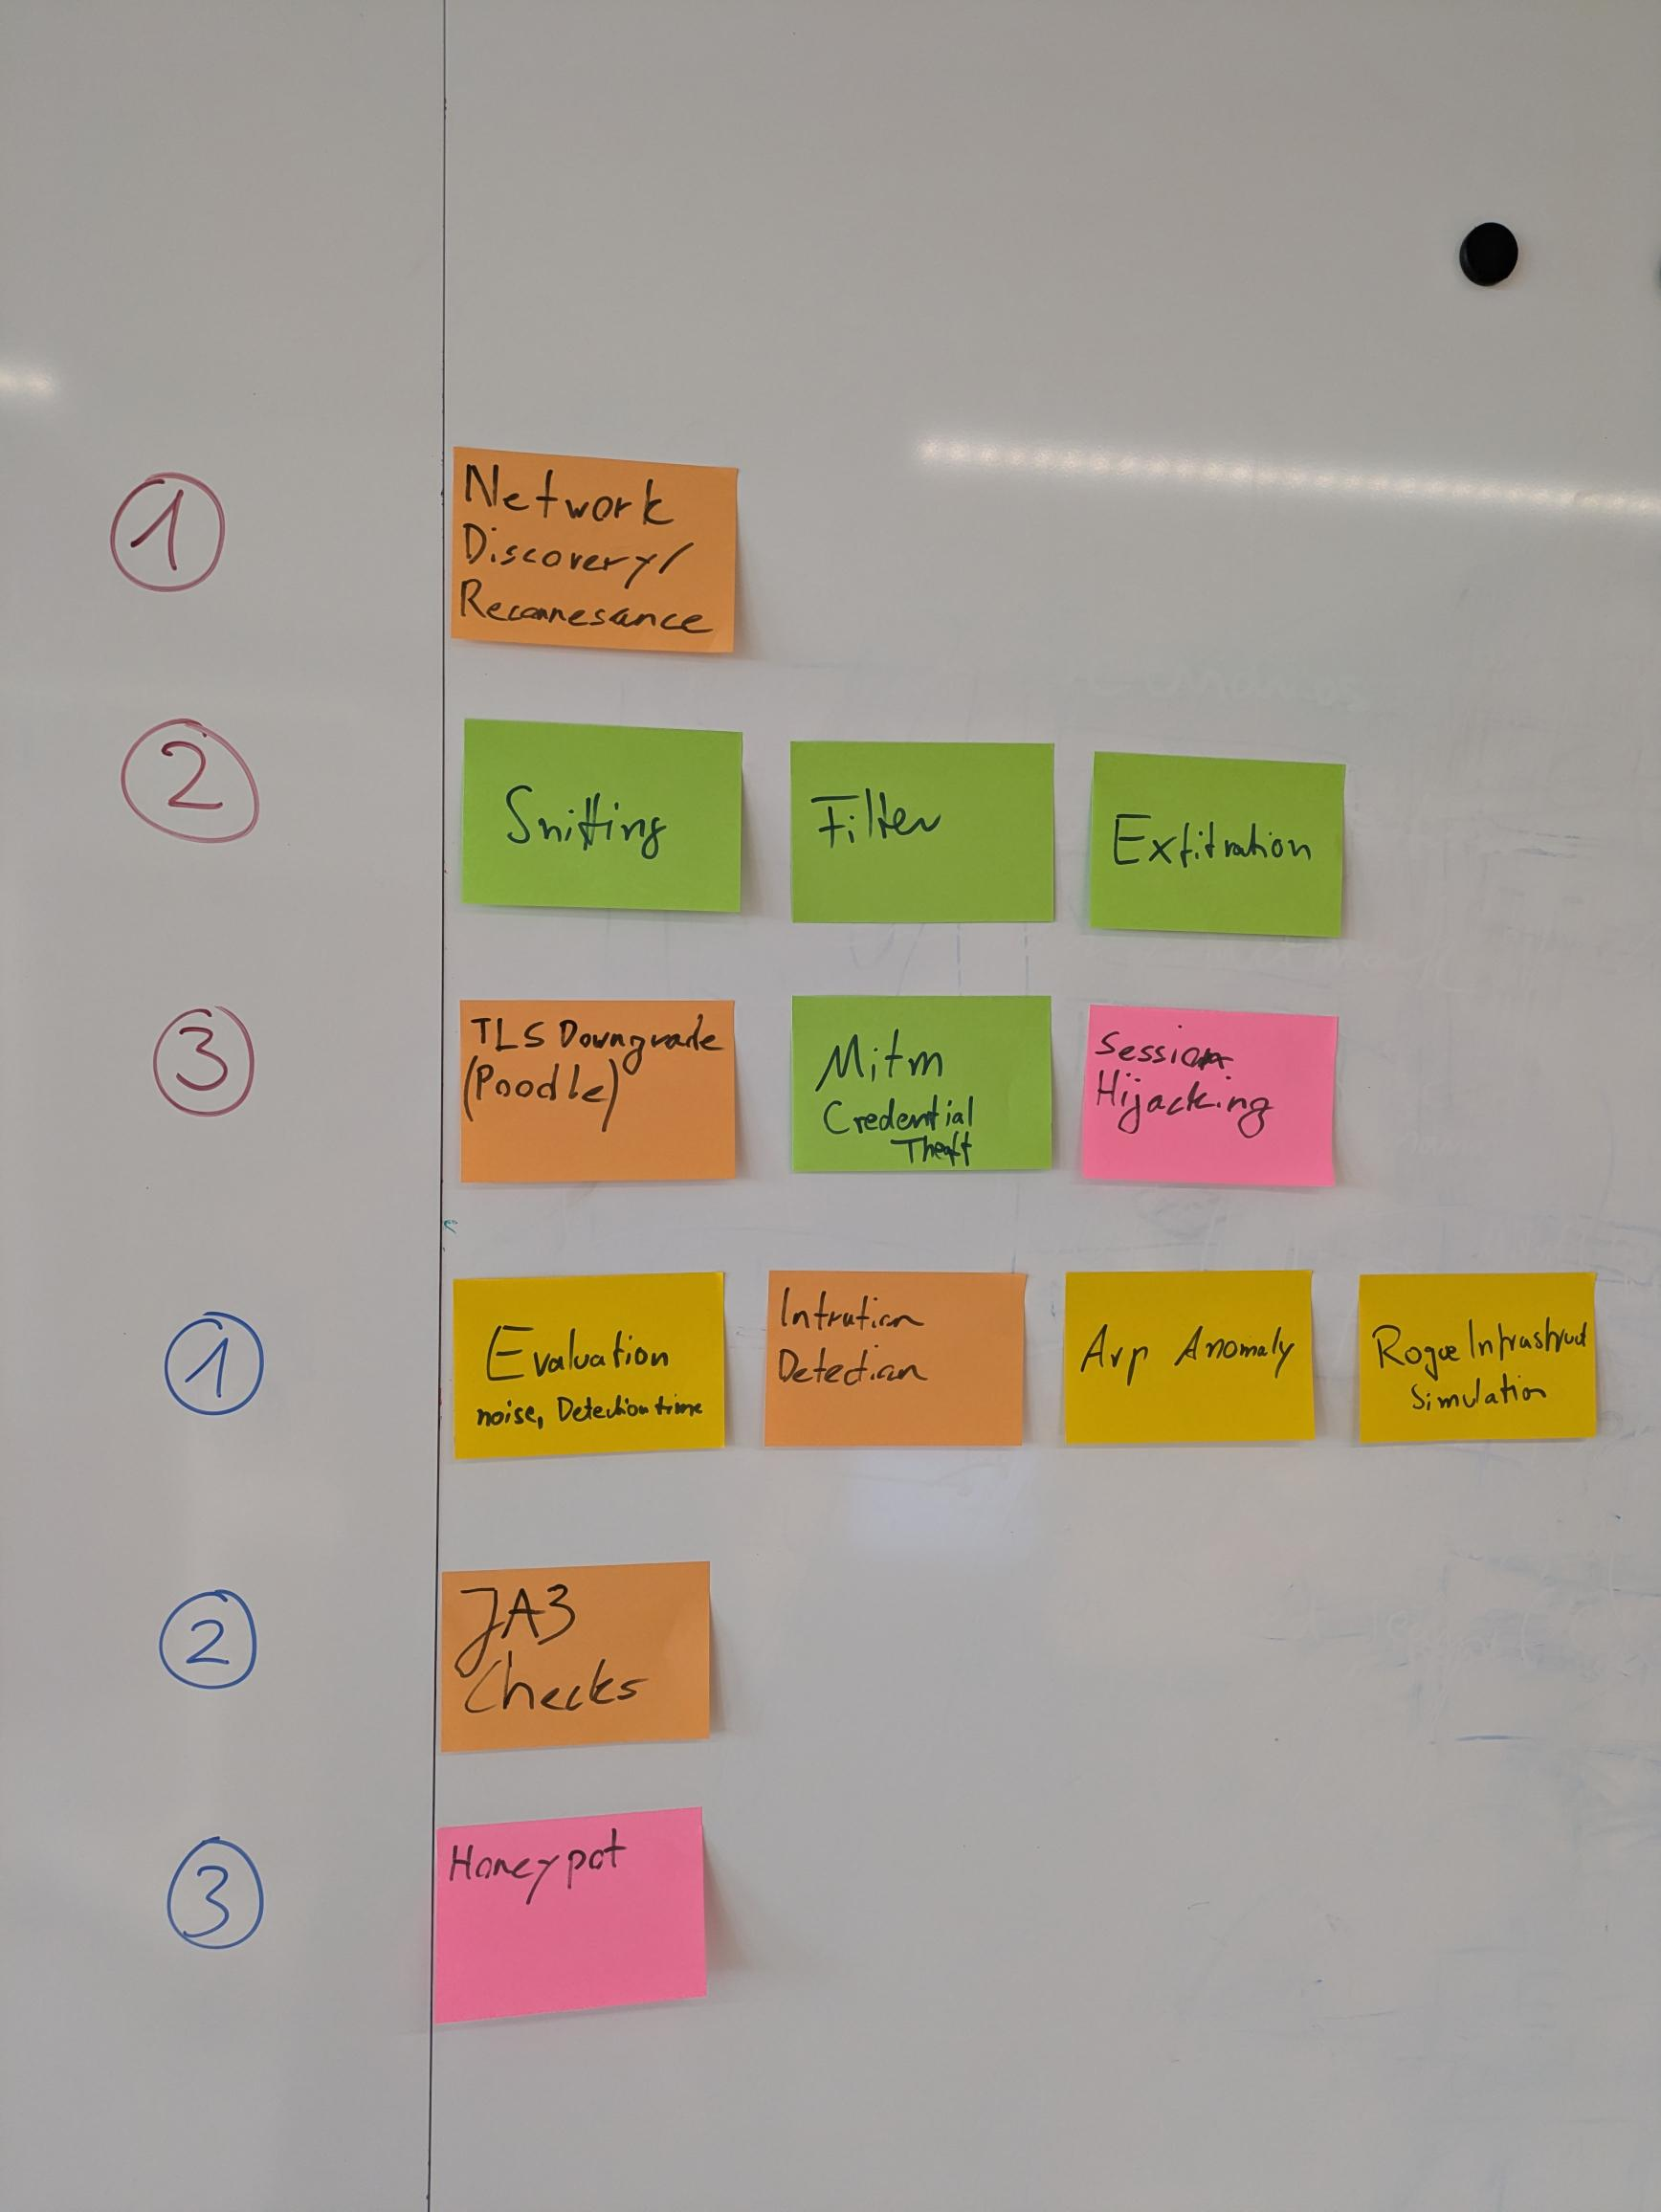
\includegraphics[width=1.0\linewidth]{appendix/appendix-media/Workshops/listing-scenarios-red-blue}
	\caption{Clustering possible Scenarios}
	\label{fig:listing-scenarios-red-blue}
\end{figure}

The Brainstorm session is used to derive further red/blue team scenarios and led to the pivot of AI-enabled Nsak scenario.

\subsection{NSAK Scenario: Network Discovery - Red Team}\label{subsec:nsak-scenario:-network-discovery---red-team}

\href{https://gitlab.ti.bfh.ch/groups/gausf1-vonal3/-/milestones/7#tab-issues}{Network Discovery Scenario}

\subsubsection{Objectives}

This workshop aims to evaluate the different steps of the network discovery process and to help participants understand how attackers identify and map potential targets within a network.

Building on this objective, Red Teams consider network discovery one of the most essential activities during the reconnaissance phase, as it helps them identify hosts and services and evaluate potential targets.
Once a network map is created, the team can use it in later phases.
For example, they might execute an ARP spoofing attack, which allows them to intercept network traffic more efficiently.

In relation to these activities, this scenario addresses the following point from the thesis proposal: \newline \enquote*{Unterstützung typischer Vorgehensweisen aus dem Red-Team- und Penetration-Testing-Bereich, etwa durch Scan- oder Angriffssimulationen.}

The workshop led to the milestone \textit{NSAK Scenario: Network Discovery – Red Team (must)}, in which each step for discovering and mapping a network is documented and structured for later implementation.

\begin{figure}[H]
	\centering
	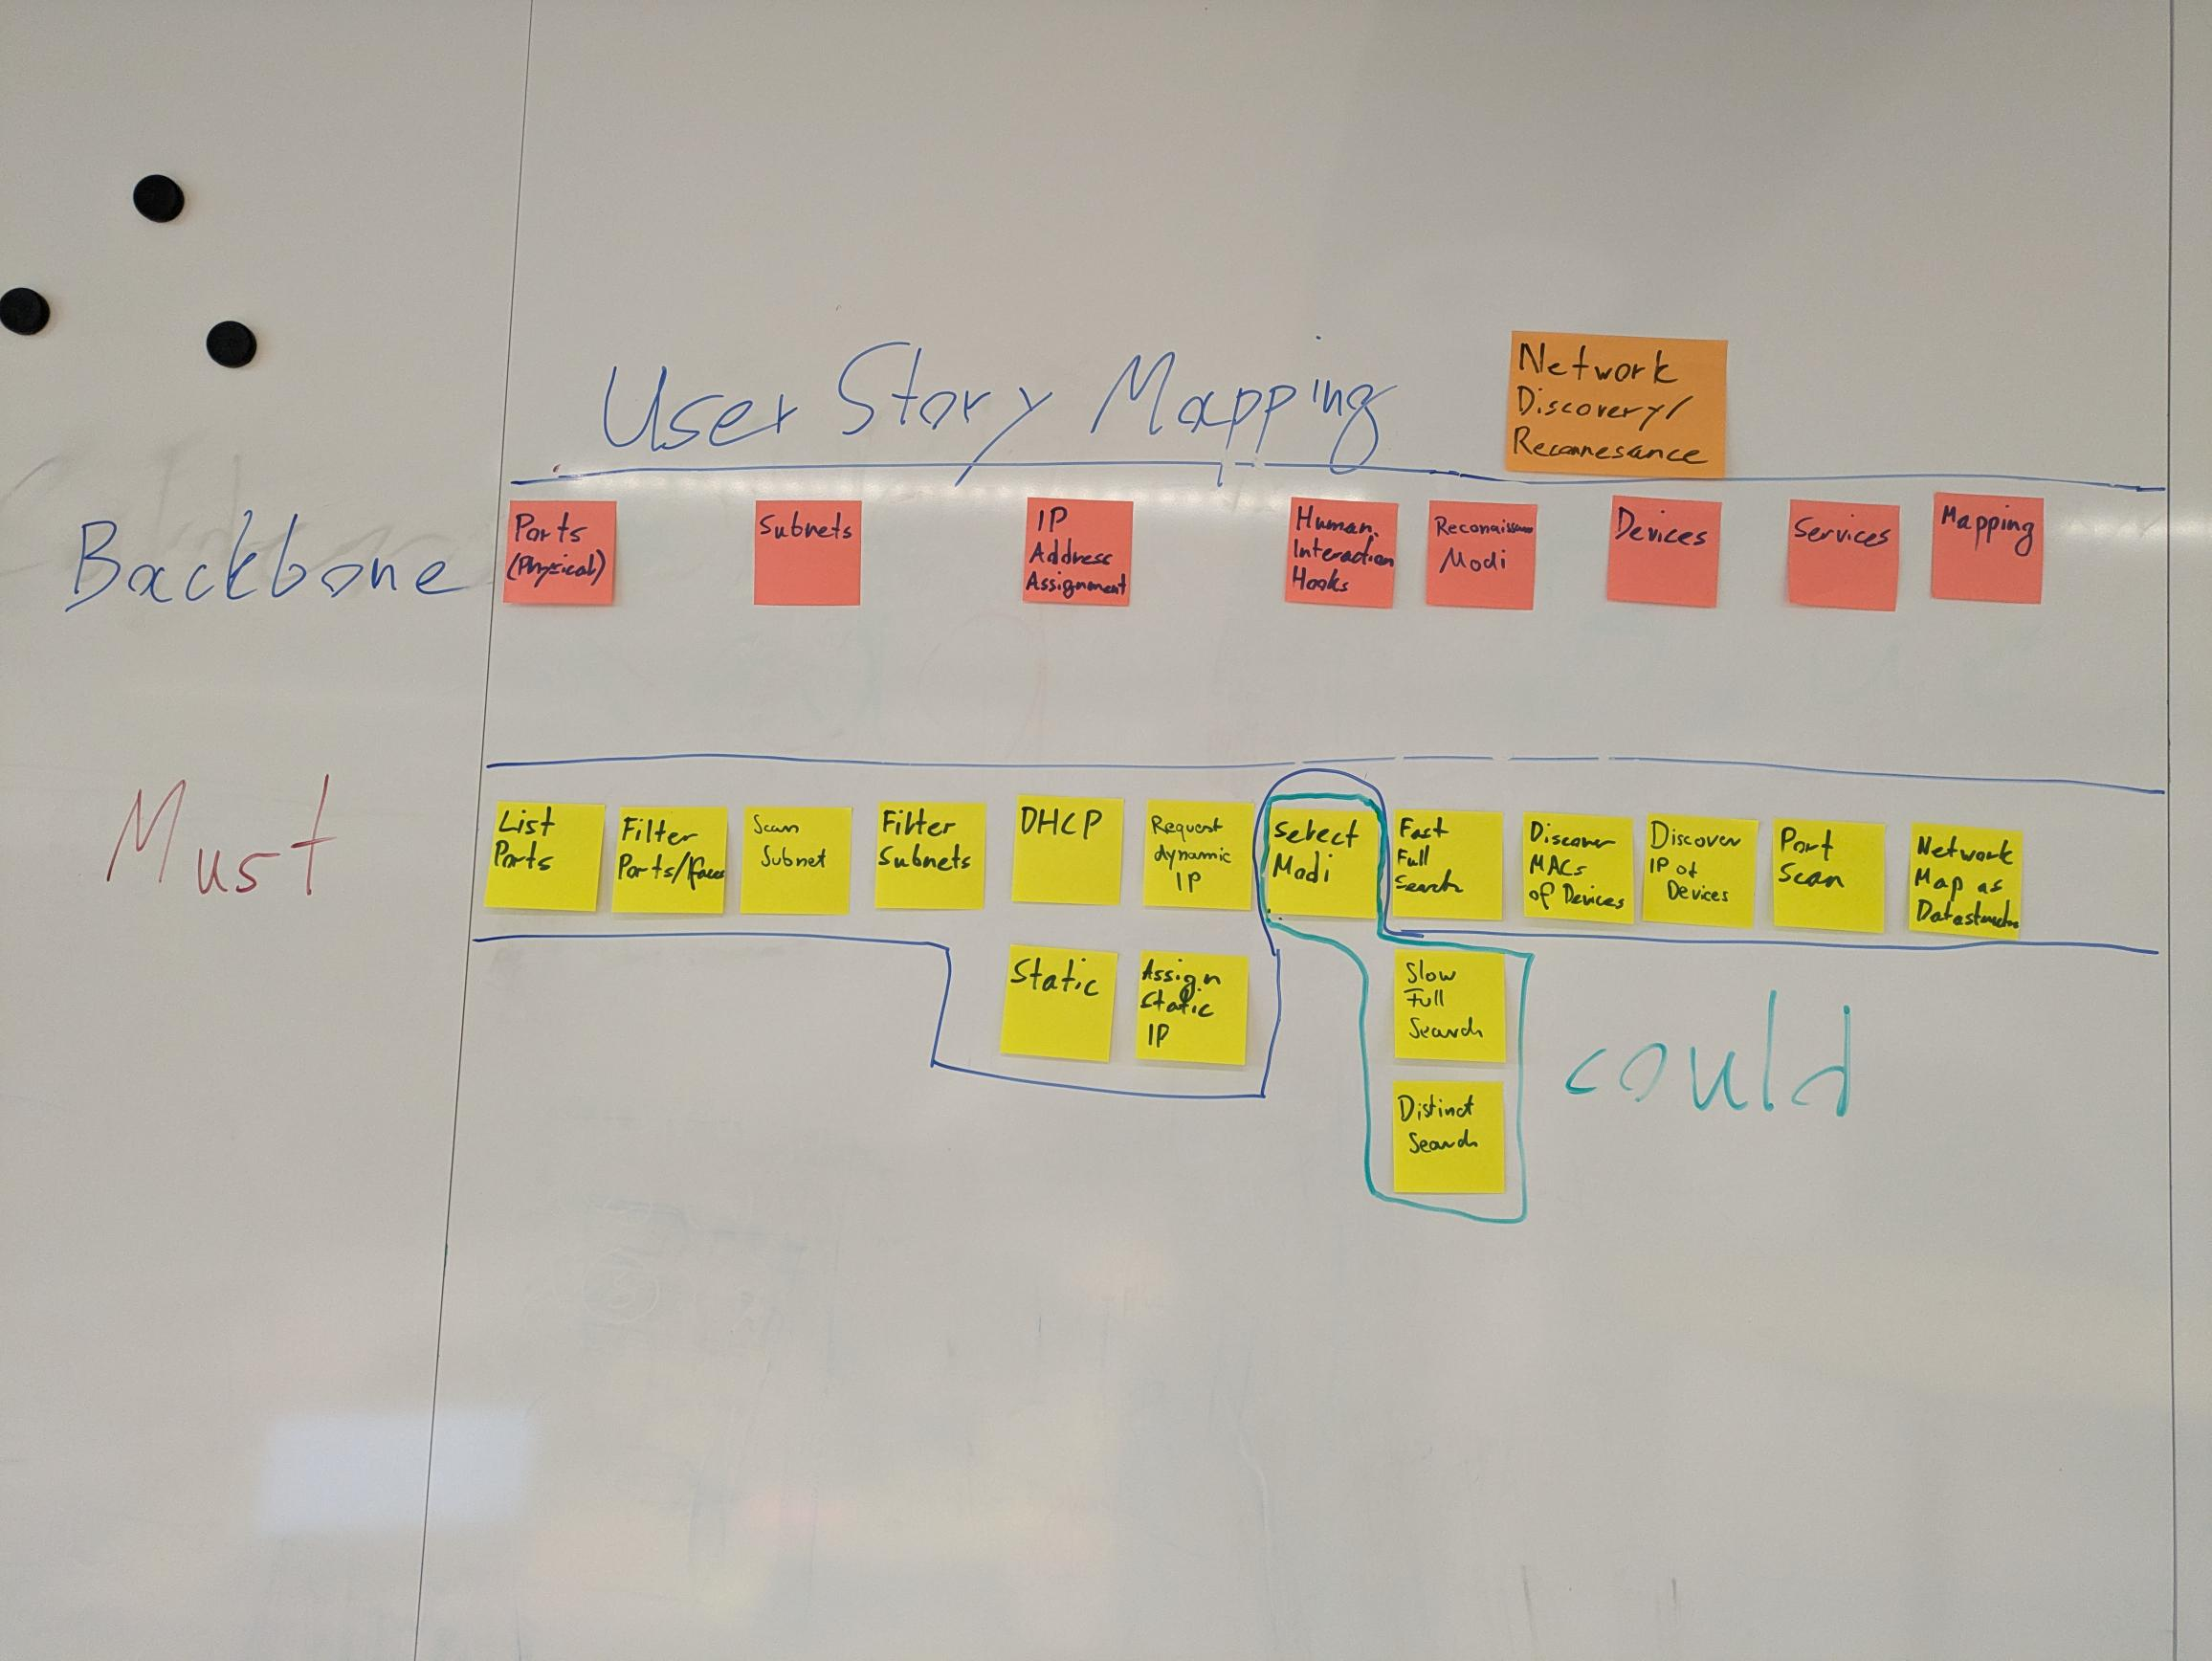
\includegraphics[width=1.0\linewidth]{appendix/appendix-media/Workshops/USM-network-discovery}
	\caption{NSAK Scenario: Network Discovery - Red Team}
	\label{fig:usm-network-discovery}
\end{figure}


\subsection{NSAK Scenario: TLS Downgrade Poodle - Red Team}\label{subsec:nsak-scenario-tls-downgrade-poodle-red-team}

\href{https://gitlab.ti.bfh.ch/groups/gausf1-vonal3/-/milestones/8#tab-issues}{TLS Downgrade Poodle Milestone}

\subsubsection{Objectives}
This workshop demonstrates how attackers can exploit TLS downgrade vulnerabilities, such as POODLE, to intercept encrypted communication.

In this scenario, the infamous POODLE attack is implemented, in which a malicious actor tries to convince a client and a server to use the vulnerable TLS version 1.1 instead of 1.2 or 1.3 to encrypt HTTP traffic.
This attack requires the attacker to sit between the client and the server (a man-in-the-middle, or MITM), allowing them to intercept and control the traffic.
When the client initiates a TLS handshake, the attacker drops packets to the server and sends TCP reset packets to the client, eventually trying older TLS versions.
Because TLS 1.1 is vulnerable to a CBC Padding attack, it is possible to create a padding oracle that gradually decrypts the cookie and hijacks the user's session.

Building on this, the scenario directly addresses the following aspect from the thesis proposal: \newline
\enquote*{Unterstützung typischer Vorgehensweisen aus dem Red-Team- und Penetration-Testing-Bereich, etwa durch Scan- oder Angriffssimulationen}


\begin{figure}[H]
	\centering
	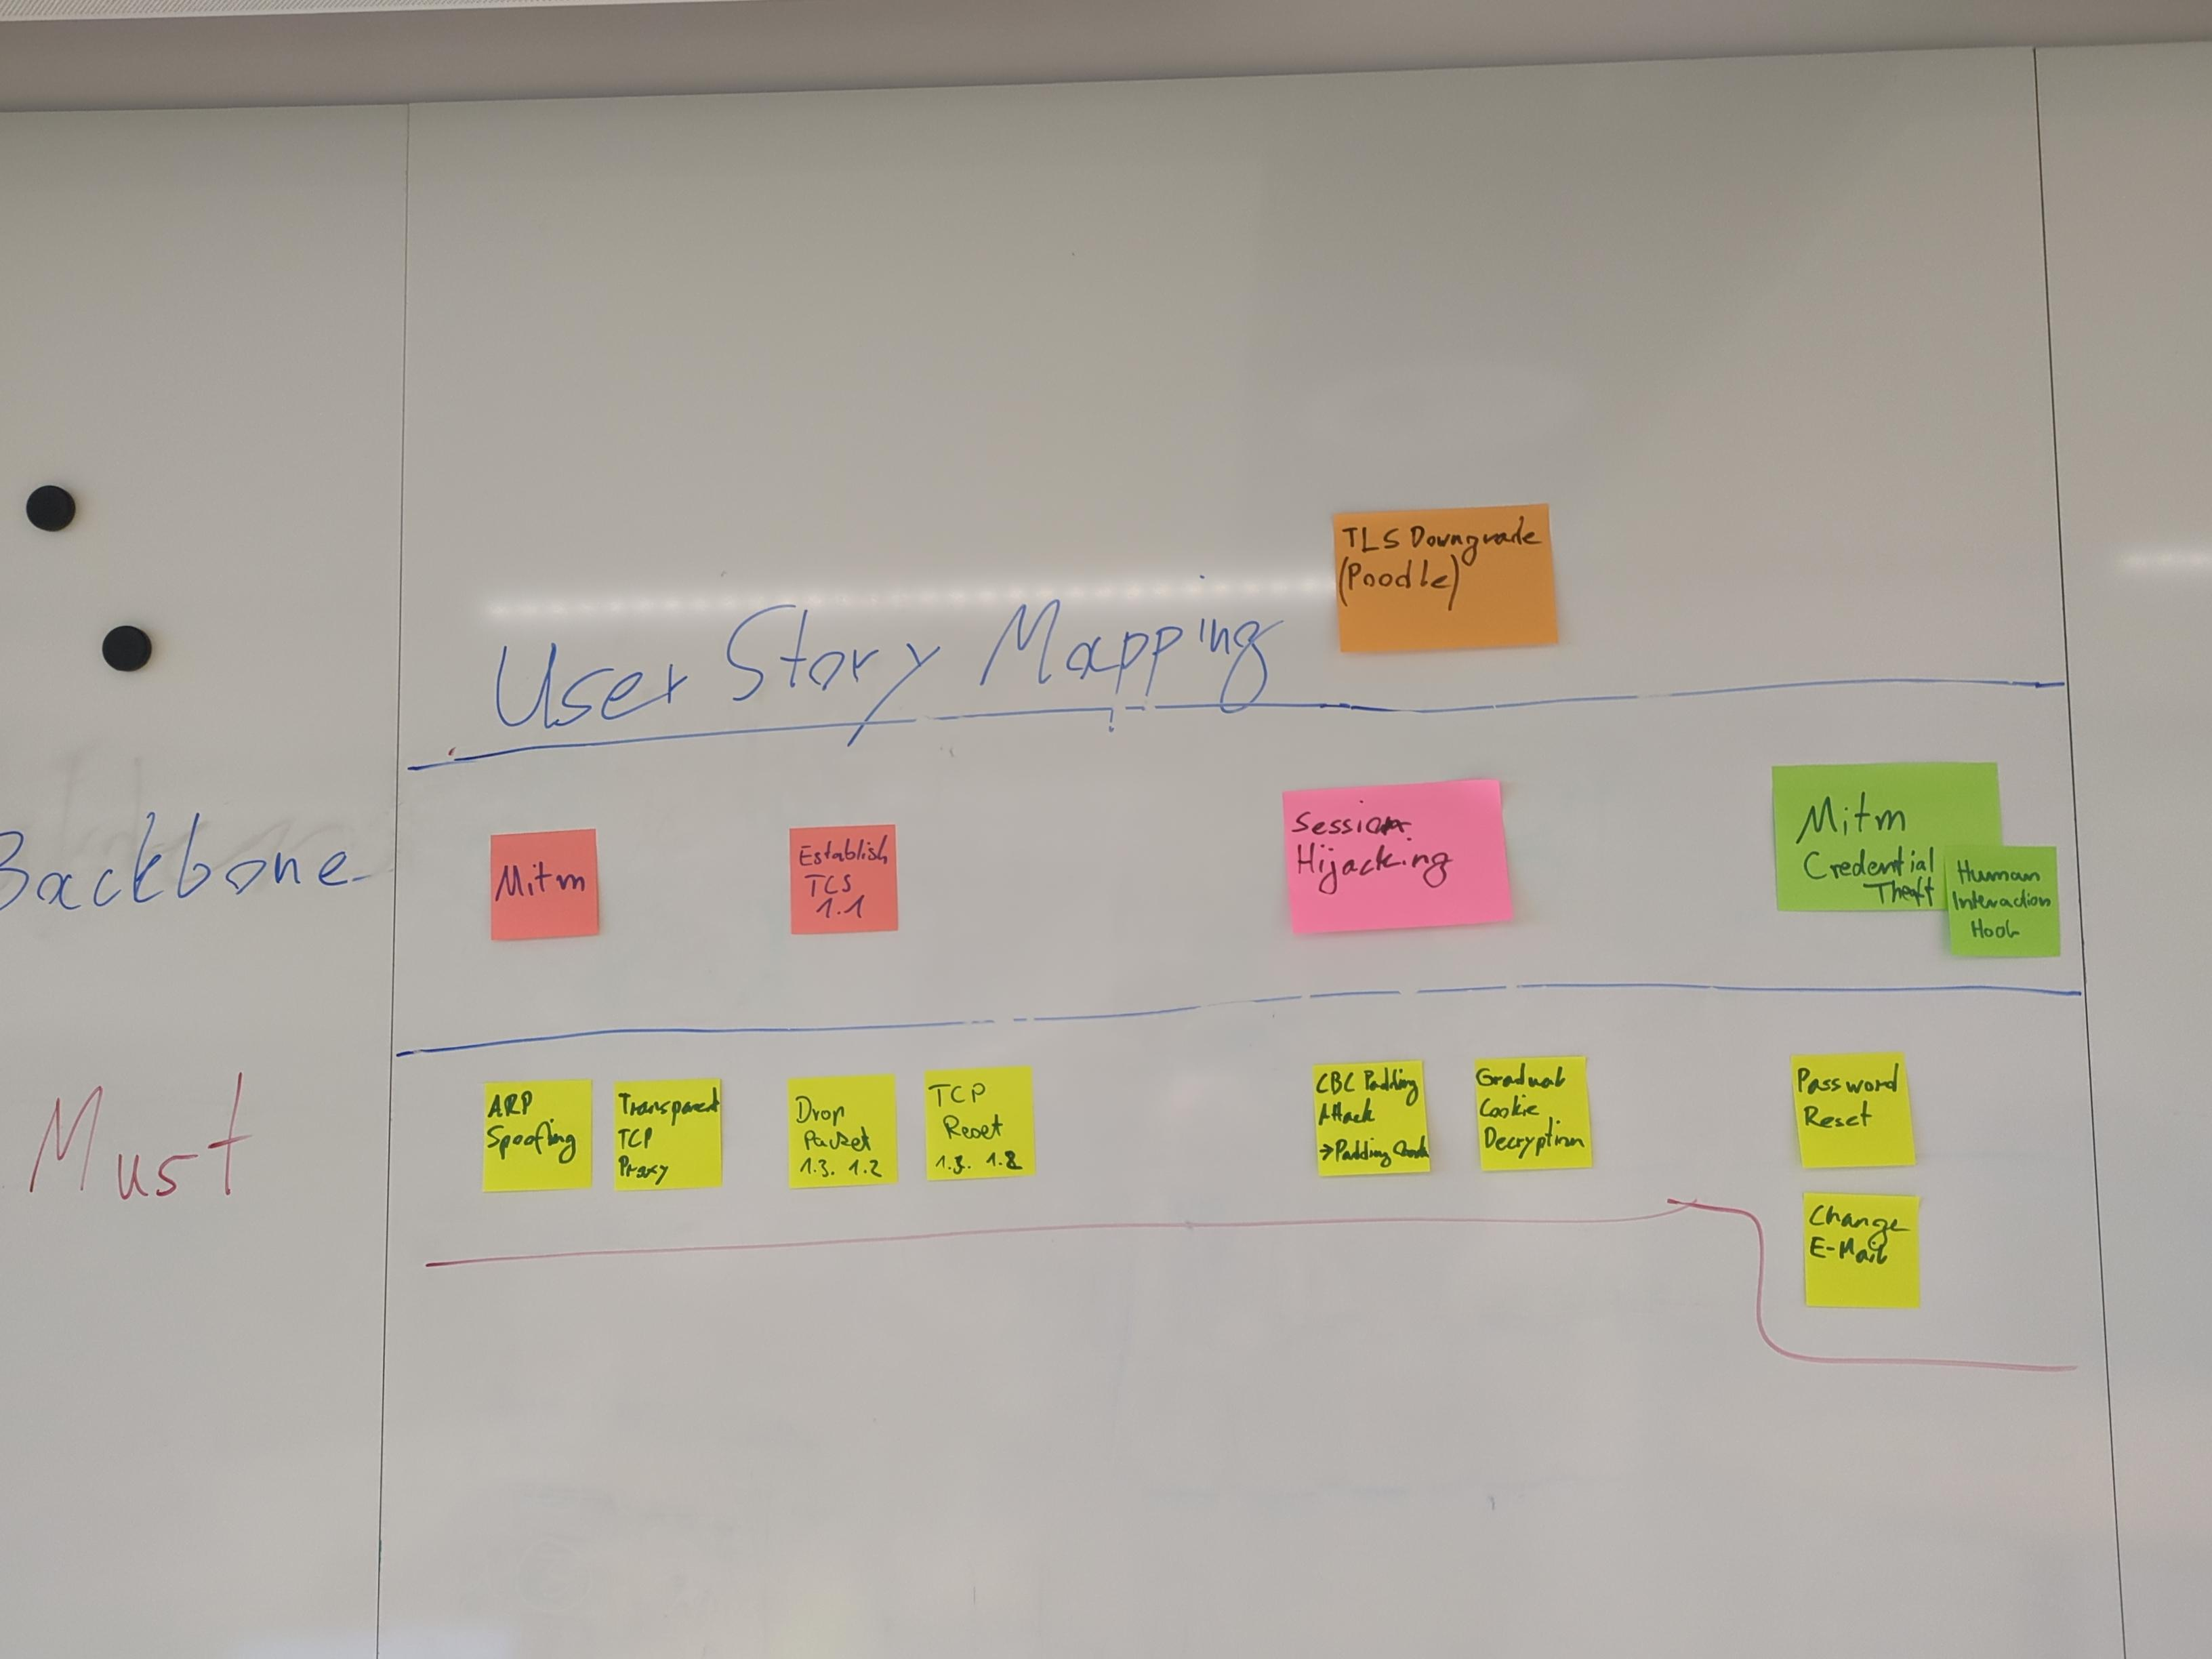
\includegraphics[width=1.0\linewidth]{appendix/appendix-media/Workshops/USM-tls-downgrade}
	\caption{NSAK Scenario: TLS Downgrade Poodle - Red Team}
	\label{fig:usm-tls-downgrade}
\end{figure}


\begin{figure}[H]
	\centering
	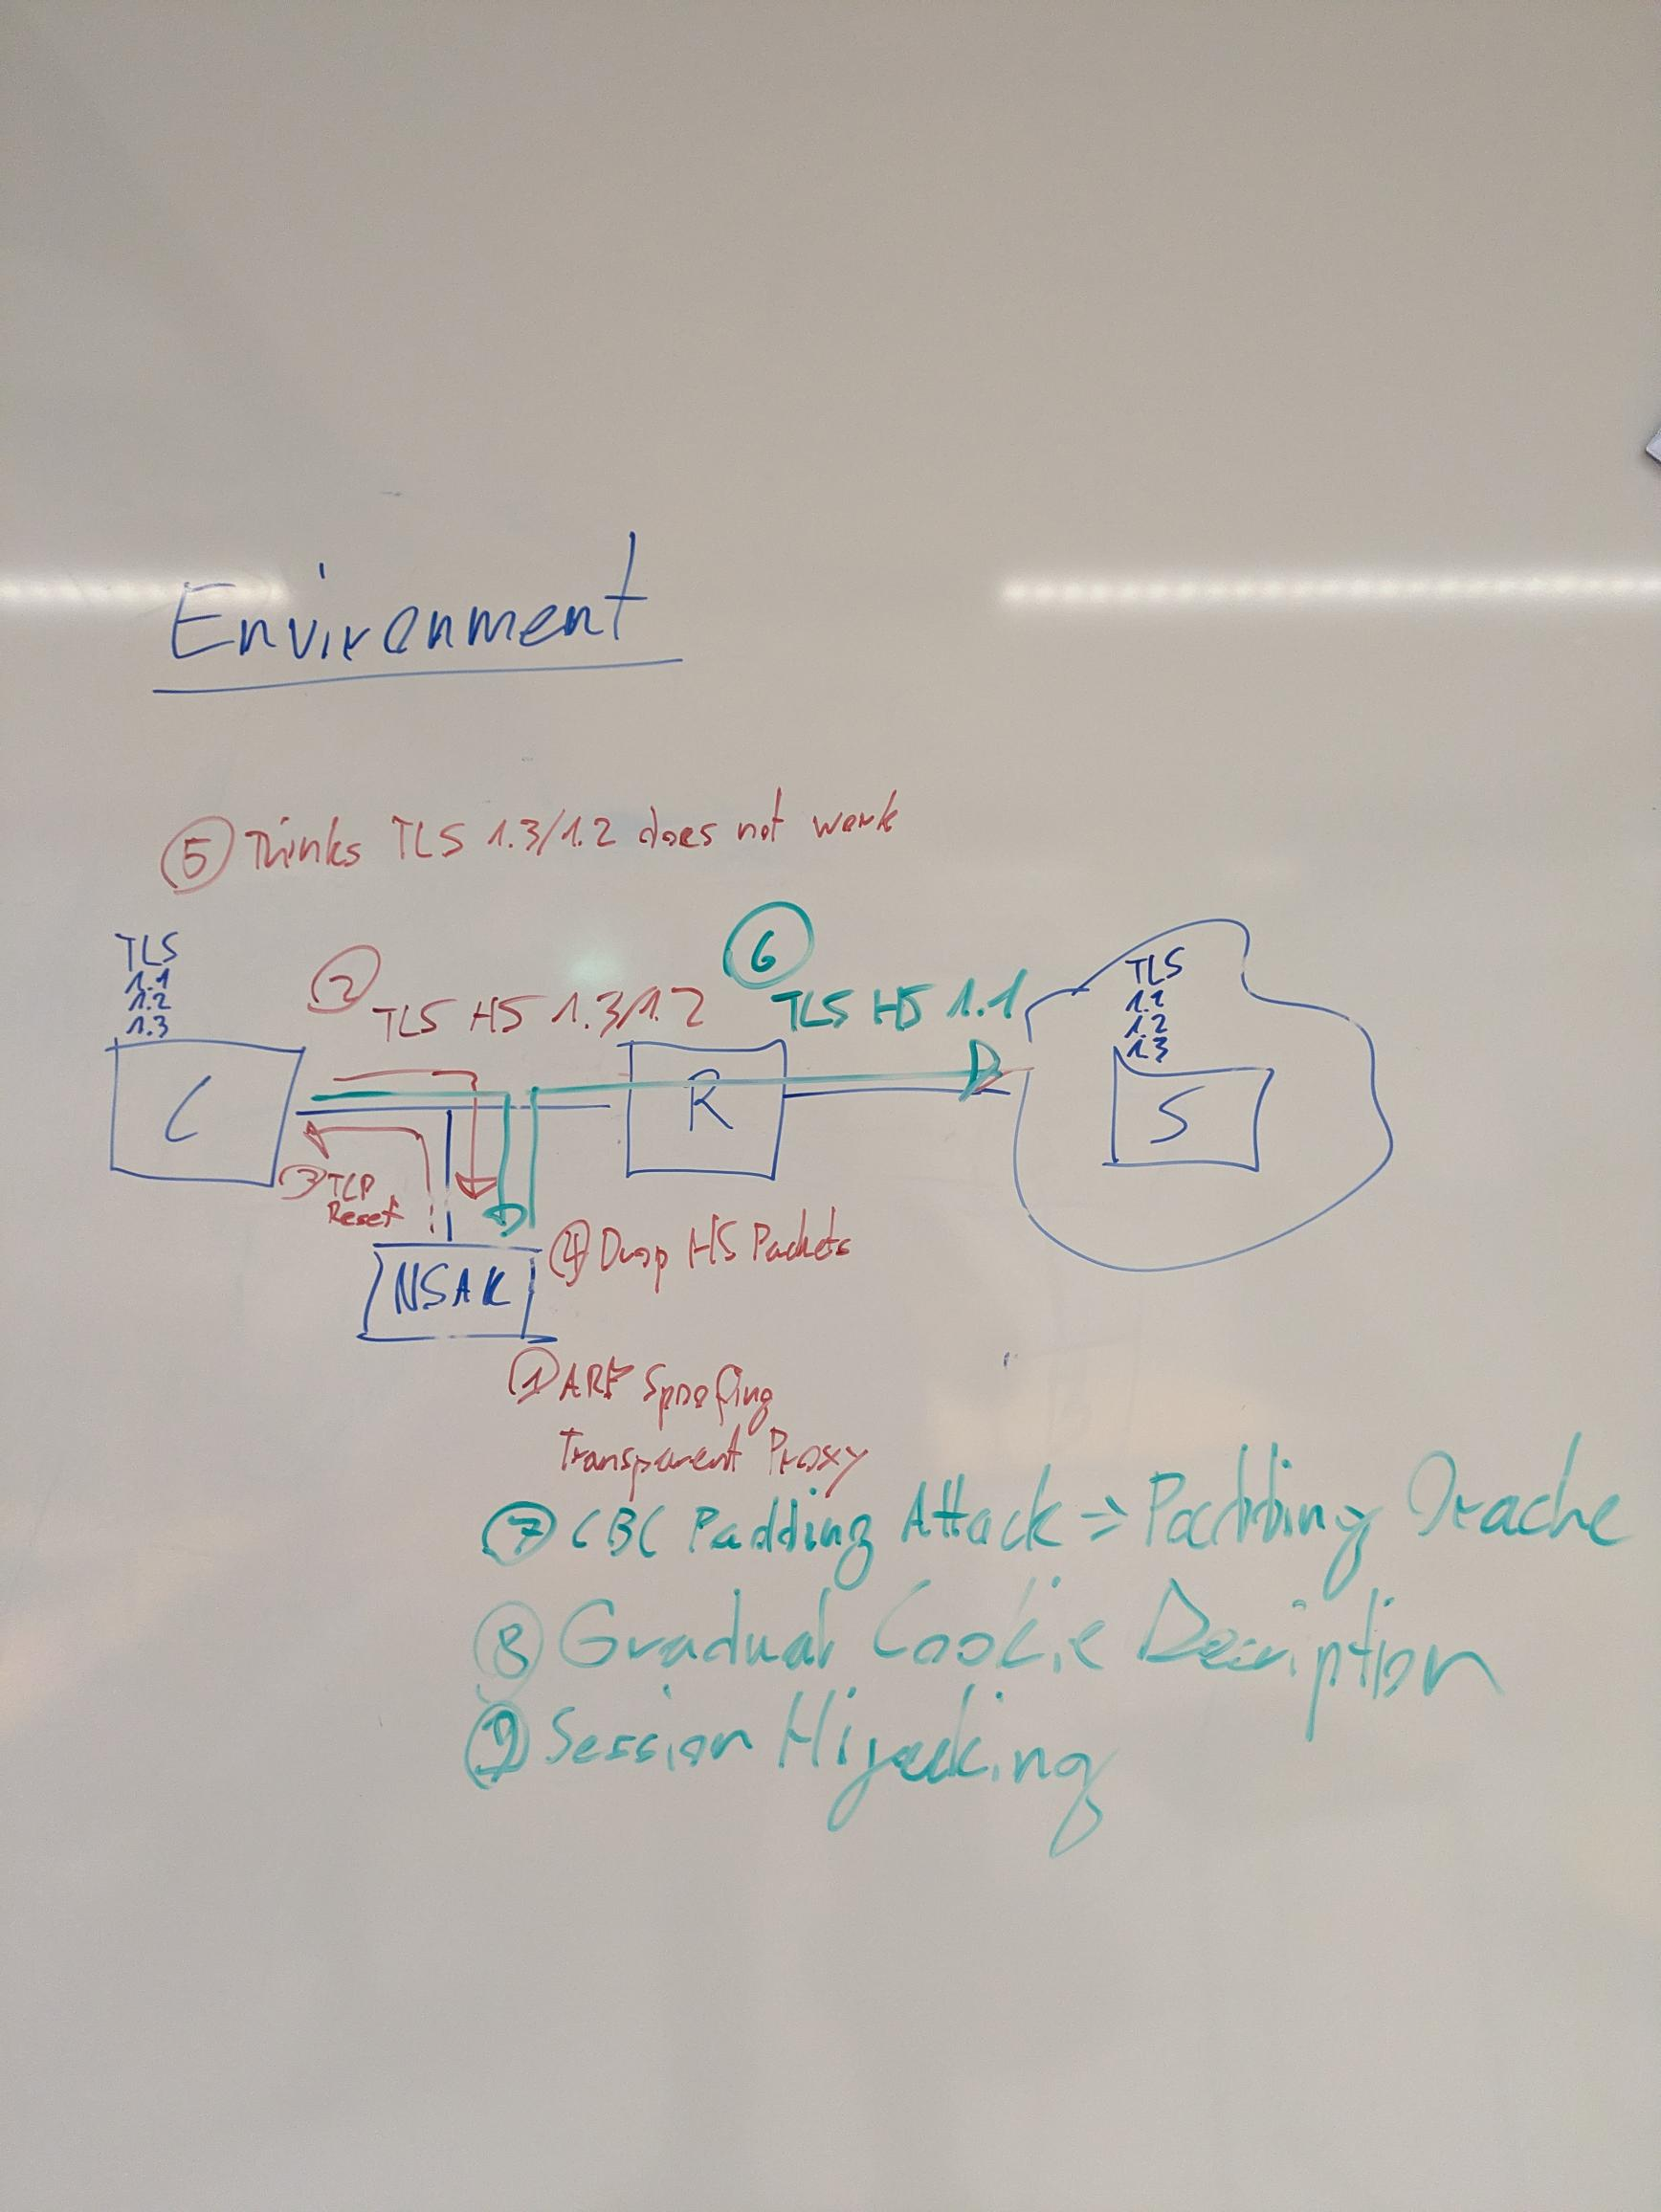
\includegraphics[width=1.0\linewidth]{appendix/appendix-media/Workshops/Environment-tls-poodle}
	\caption{NSAK Scenario: TLS Downgrade Poodle -Topology}
	\label{fig:environment-tls-poodle}
\end{figure}



\subsection{NSAK Scenario: Honeypot - Blue Team}\label{subsec:nsak-scenario:-honeypot-blue-team}

\href{https://gitlab.ti.bfh.ch/groups/gausf1-vonal3/-/milestones/14#tab-issues}{Honeypot Milestone}

Honeypots can serve as an additional form of intrusion detection and help Blue Teams detect attackers in a network.
The system tries to attract malicious actors by providing an attack surface as large as possible; a simple way to achieve this is to open ports.
After an attacker tries to connect to any of the open ports, the system notifies an operator and may close all open ports to prevent further attempts to compromise the Honeypot.
The operator can then manually intervene to identify and isolate the attacker and analyze the captured payload.

This scenario covers the following bullet point from the thesis proposal: \newline
\enquote*{Bereitstellung von Funktionen zur Erkennung, Protokollierung und Analyse verdächtiger Aktivitäten als Teil defensiver Massnahmen}

\begin{figure}[H]
	\centering
	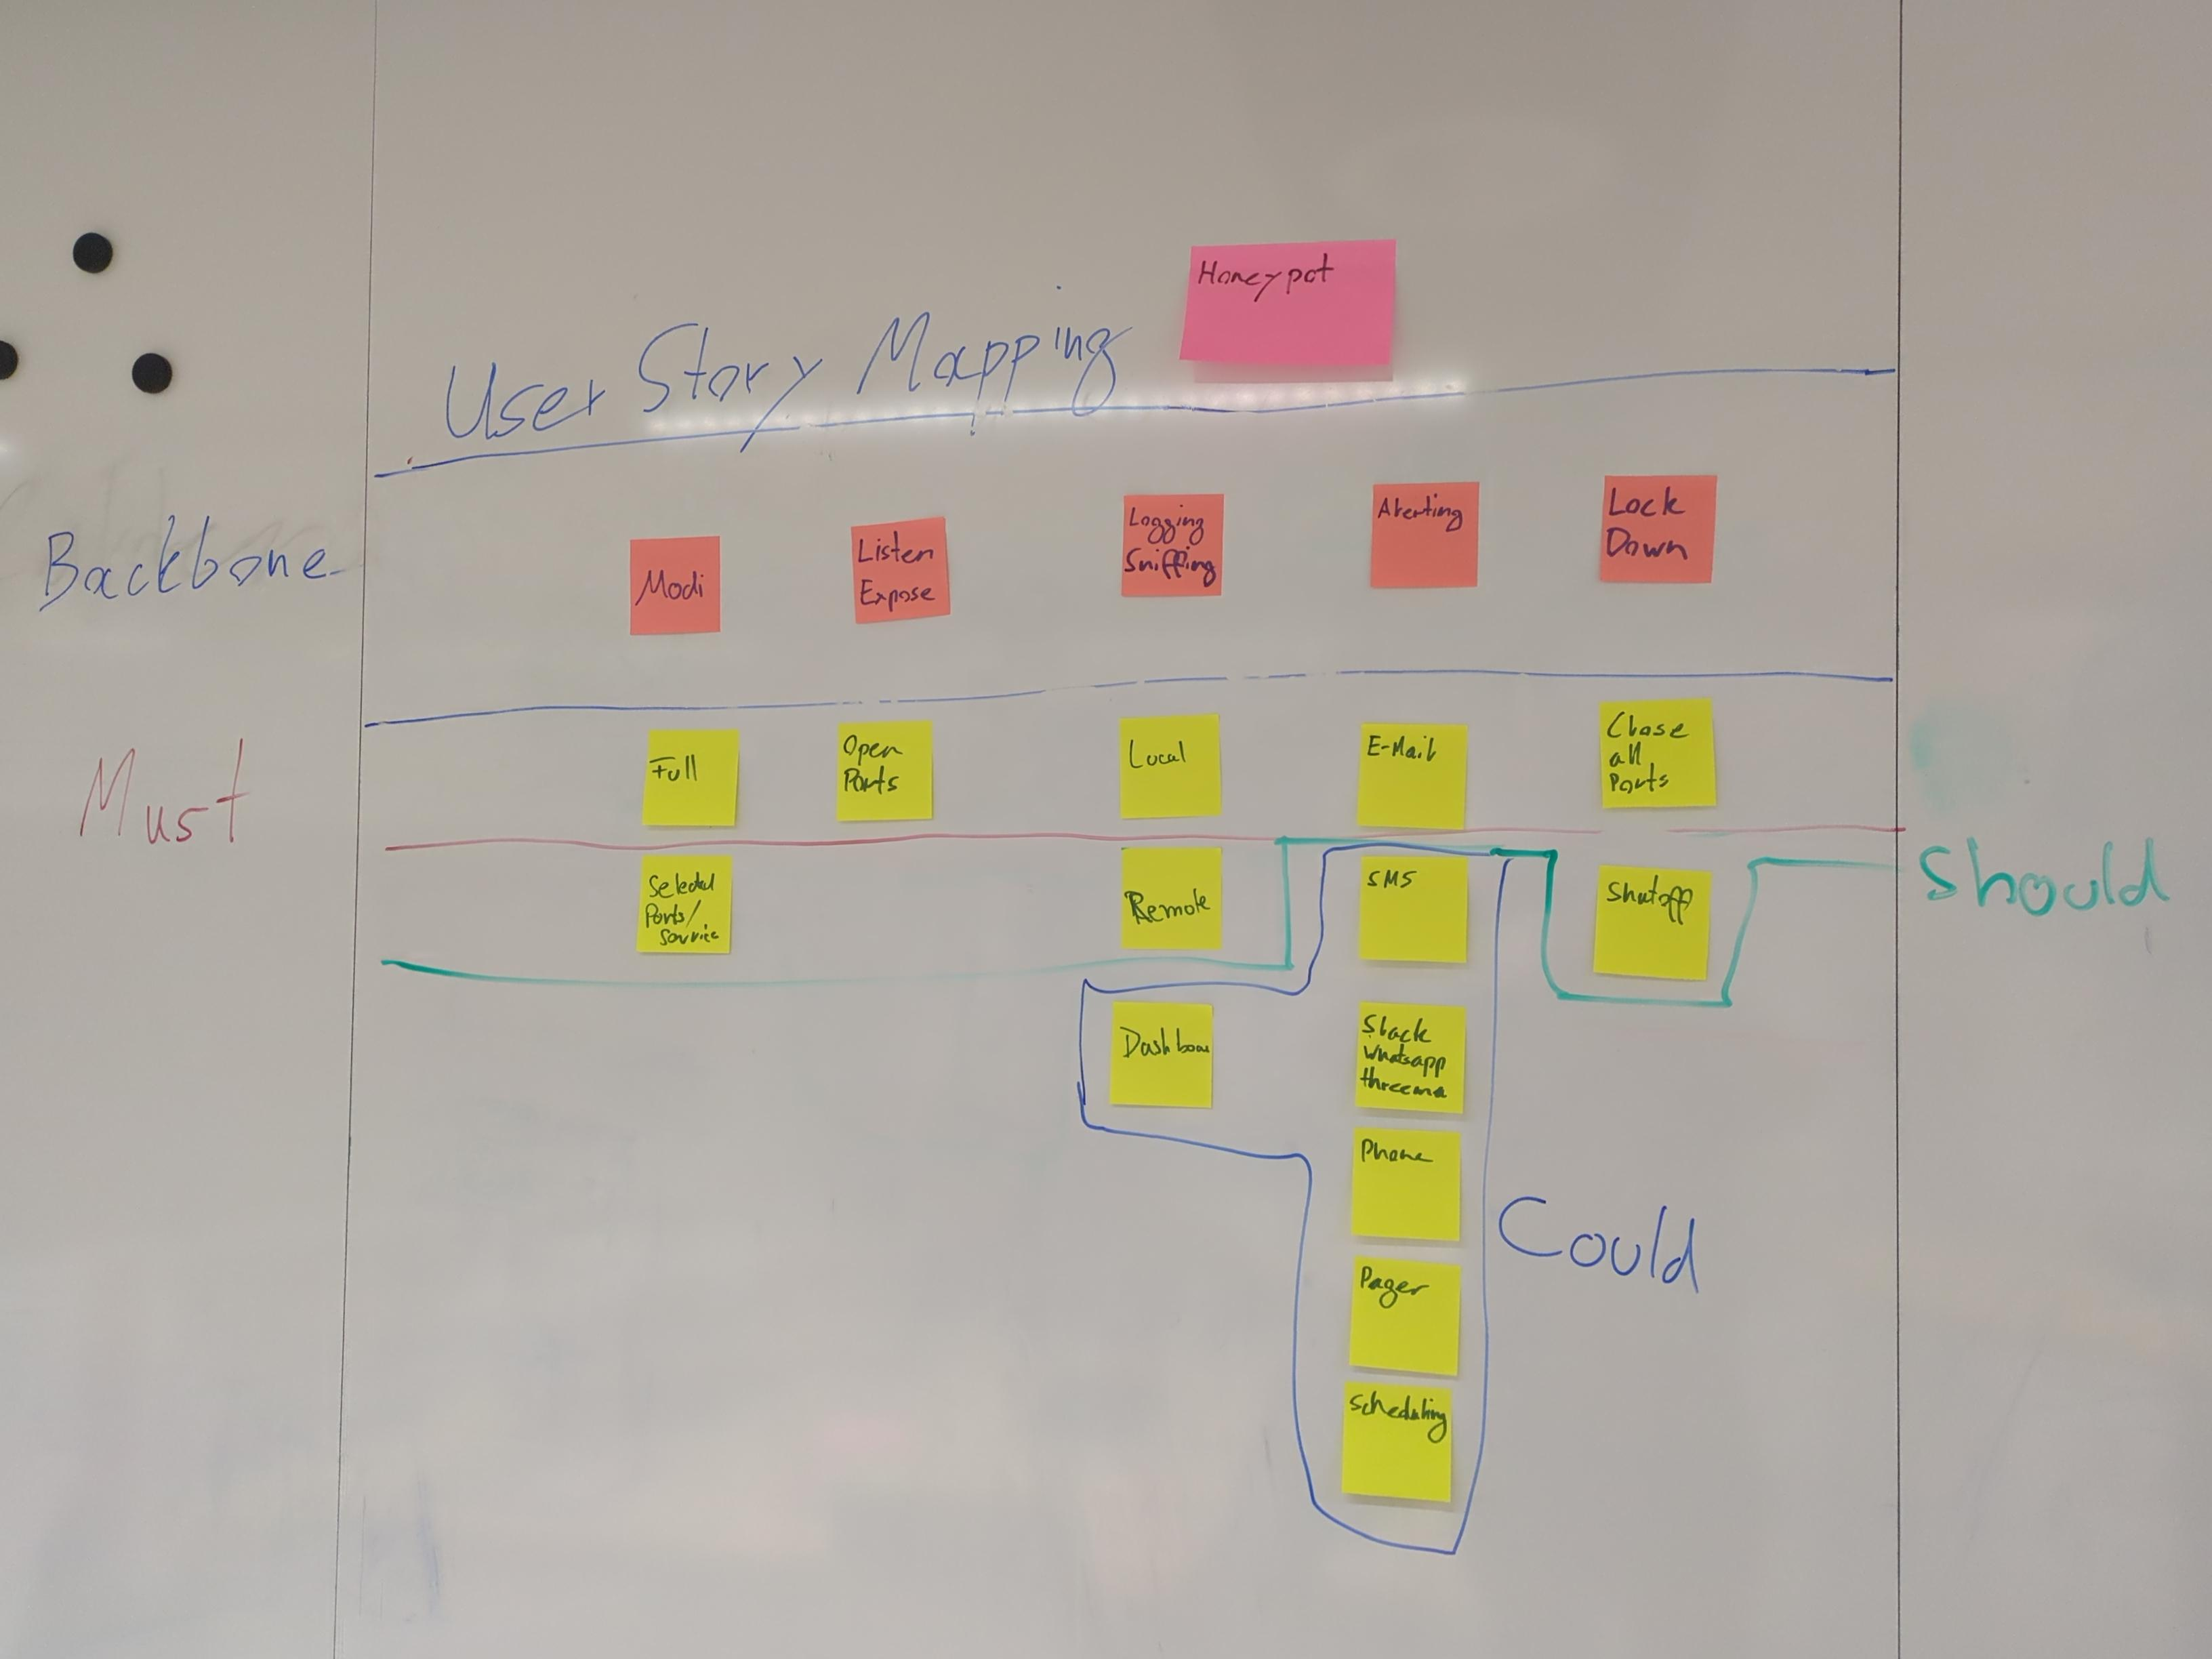
\includegraphics[width=1.0\linewidth]{appendix/appendix-media/Workshops/USM-honeypot}
	\caption{NSAK Scenario: Honeypot - Blue Team}
	\label{fig:usm-honeypot}
\end{figure}

\subsection{NSAK Scenario: Traffic Capture - Red Team}\label{subsec:nsak-scenario:-traffic-capture-red-team}

\href{https://gitlab.ti.bfh.ch/groups/gausf1-vonal3/-/milestones/6#tab-issues}{Traffic Capture Milestone}

Capturing, exfiltrating, and analyzing traffic from a targeted network is a key Red Team activity and crucial for initial reconnaissance and planning the next phases of the attack.
Based on the gathered intelligence, network participants and services can be identified, and possible attack vectors may be evaluated.
If unencrypted traffic is present on the network, session data and credentials could already have been extracted.

This scenario addresses the following bullet point from the thesis proposal:
\enquote*{Untersuchung und Auswertung der Netzwerkkommunikation zwischen Endgeräten und externen Netzen.}
\begin{figure}[H]
	\centering
	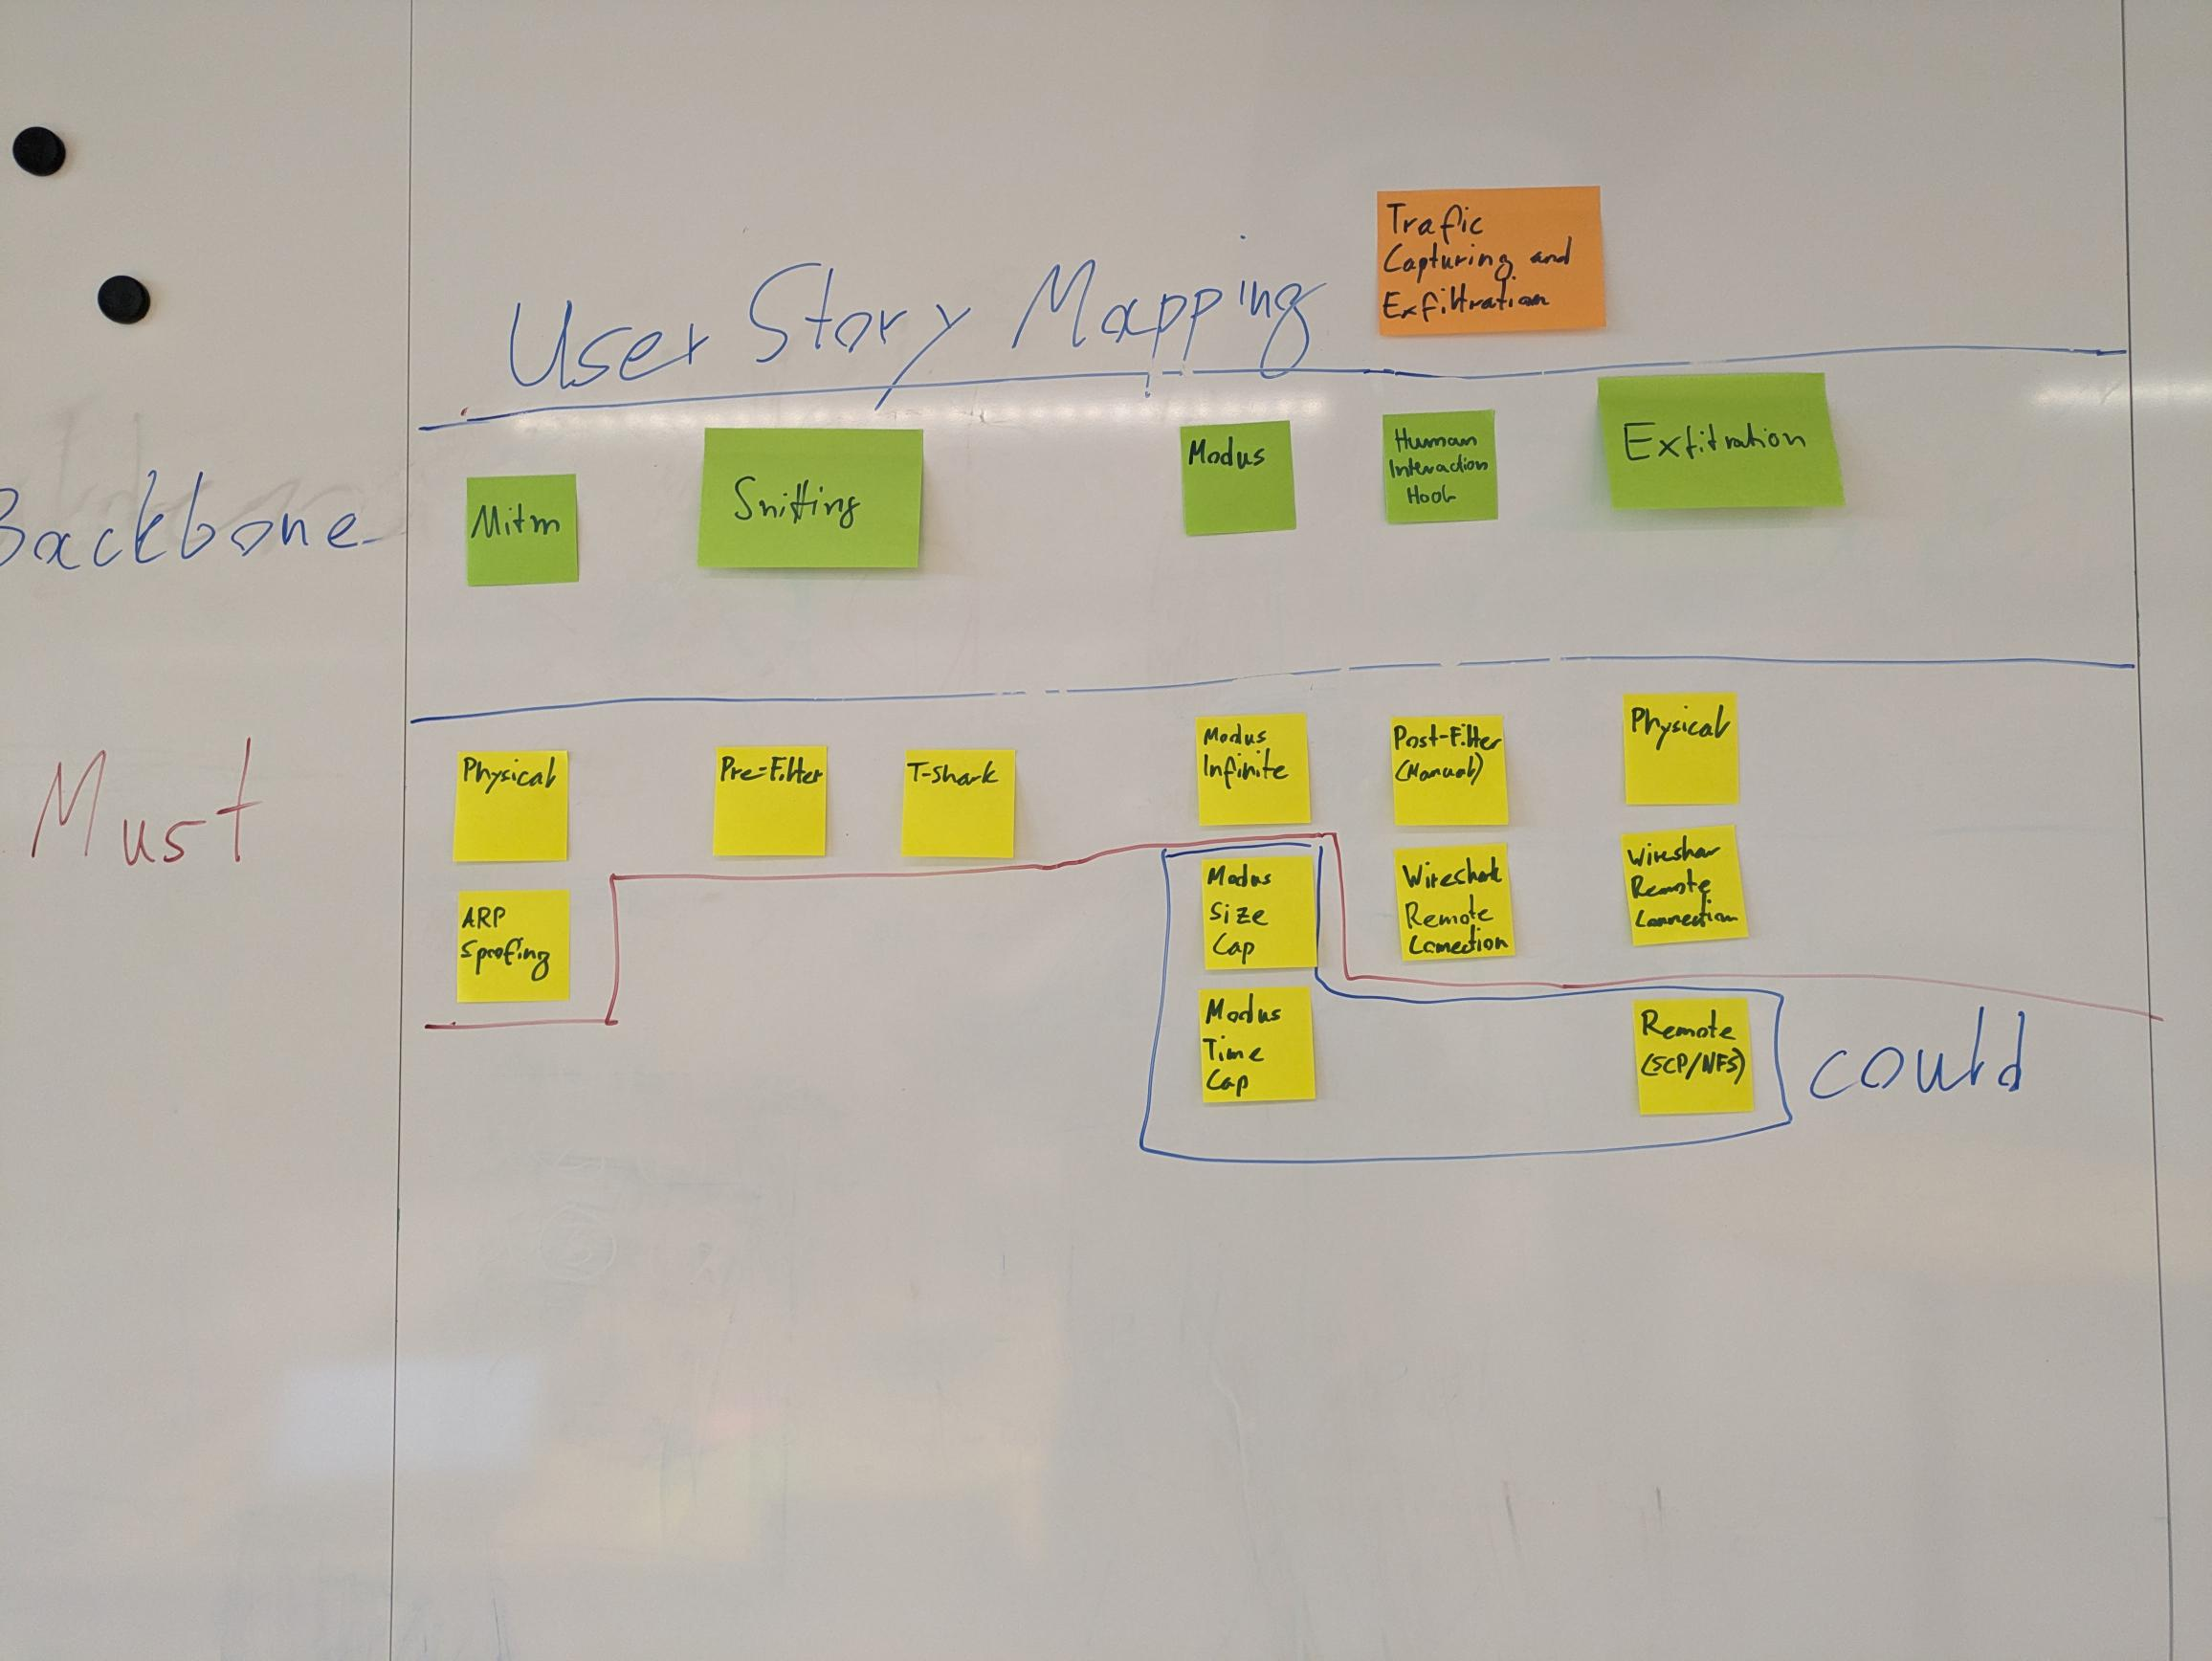
\includegraphics[width=1.0\linewidth]{appendix/appendix-media/Workshops/USM-traffic-capture}
	\caption{NSAK Scenario: Traffic Capture - Red Team}
	\label{fig:usm-traffic-capture}
\end{figure}

\subsection{NSAK Scenario: Intrusion Detection - Blue Team}\label{subsec:nsak-scenario:-intrusion-detection-blue-team}

\href[]{https://gitlab.ti.bfh.ch/groups/gausf1-vonal3/-/milestones/13#tab-issues}{Intrusion Detection Milestone}

Intrusion detection is one of the core Blue Team activities and aims to identify malicious actors and misconfigured clients in production network environments.
This can be achieved by introducing a system at a traffic mirroring port or as a central point in a network.
The intrusion detection system can leverage a wide array of security policies, reference traffic, and other markers to effectively identify anomalies.
As soon as suspicious activity is detected or a policy is violated, automated measures may be initiated, and security engineers will be automatically alerted for manual intervention.

This scenario covers the following bullet point from the thesis proposal: \enquote{Bereitstellung von Funktionen zur Erkennung, Protokollierung und Analyse verdächtiger Aktivitäten als Teil defensiver Massnahmen}

\begin{figure}[H]
	\centering
	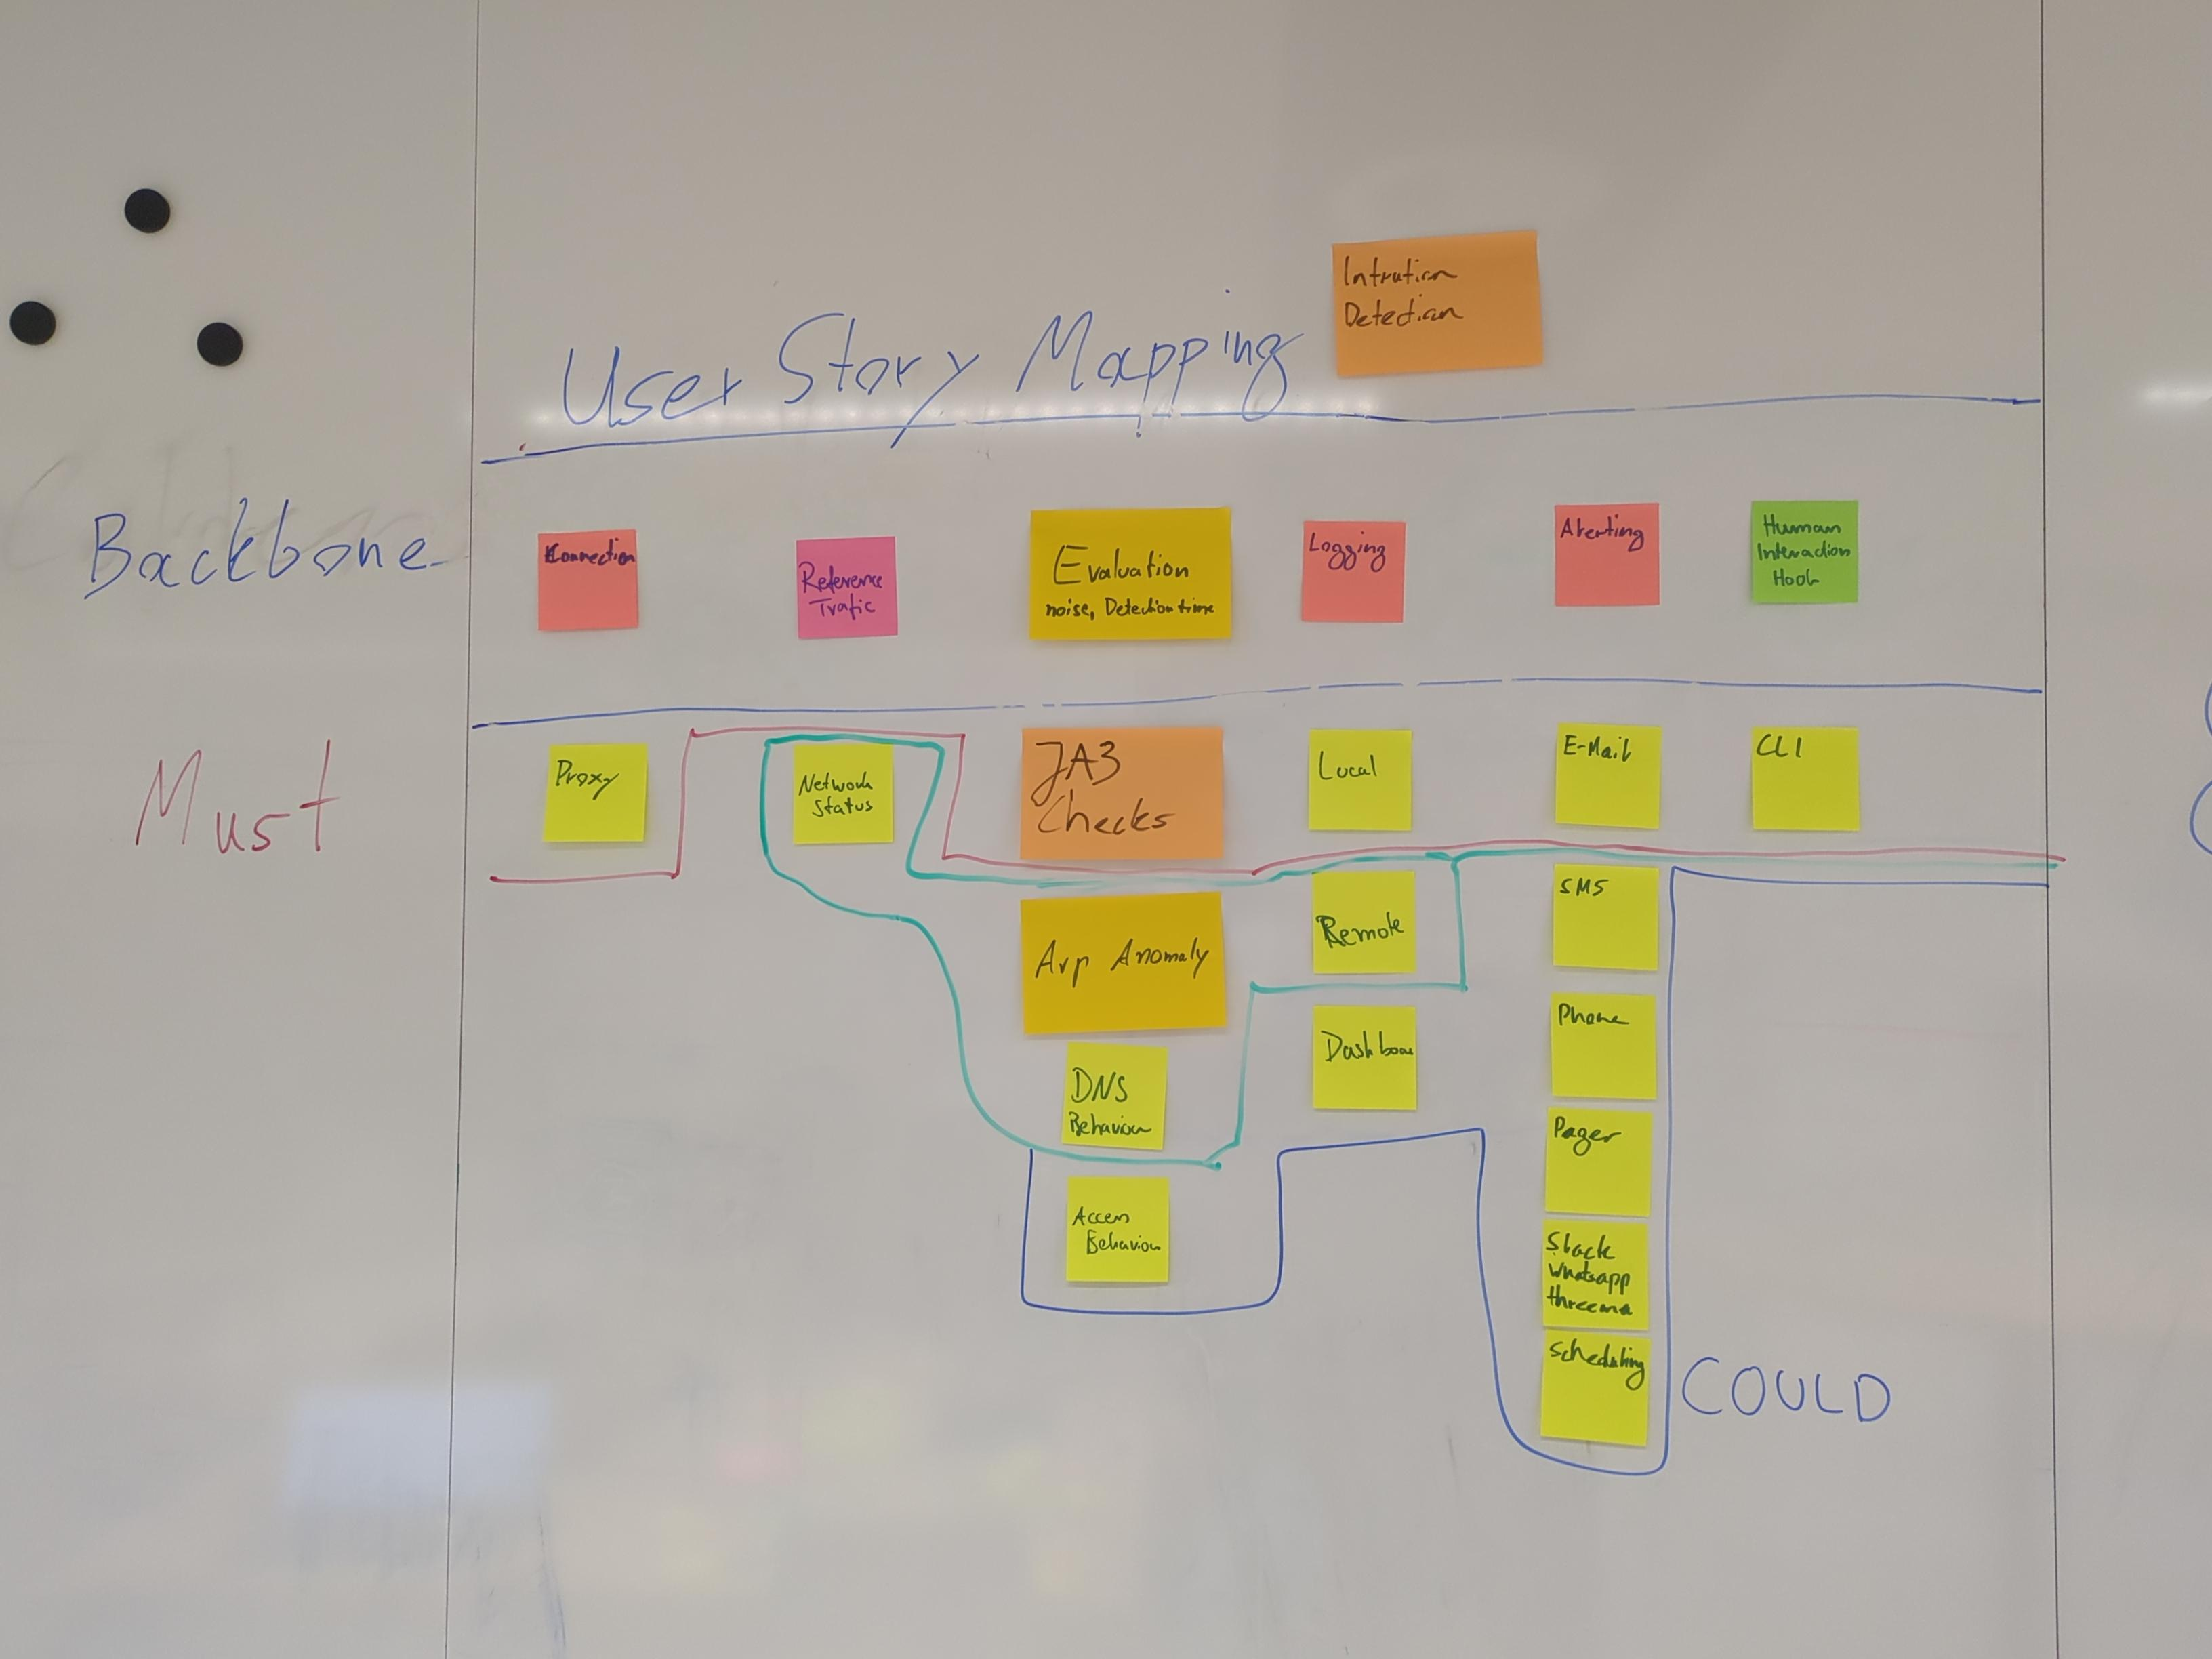
\includegraphics[width=1.0\linewidth]{appendix/appendix-media/Workshops/USM-intrusion-detection}
	\caption{NSAK Scenario: Intrusion Detection - Blue Team}
	\label{fig:usm-intrusion-detection}
\end{figure}
